
\section{Structured Litterature Study}

  \subsection*{Planning}

    This section will give a detailed plan for the structured litterature review, as well as building a 
    evaluation protocol for the review. 
    Research should be conducted in order to answer questions that have not been answerd yet. 
    By conducting a structured literature review, I can support my motivation for doing the research, 
    as well as get to know relevant research. 

    \subsection*{Field of Study}

      Before conducting the litterature study, I will do a specification of my field of study in order to
      avoid a unsustainable broad scope. Too broas scope in a litterature study can give to irrelevant searches 
      and it will be hard to find the relevant information needed to answer the research questions. 

      In the figure below I have done a analysis of my field of study. The research will focus on authentication on mobile devices. 
      The type of authentication is screen locks. Finally the inner circle, the most specific topic, is the Android Unlock Pattern. 

      \begin{figure}[H]
        \centering
        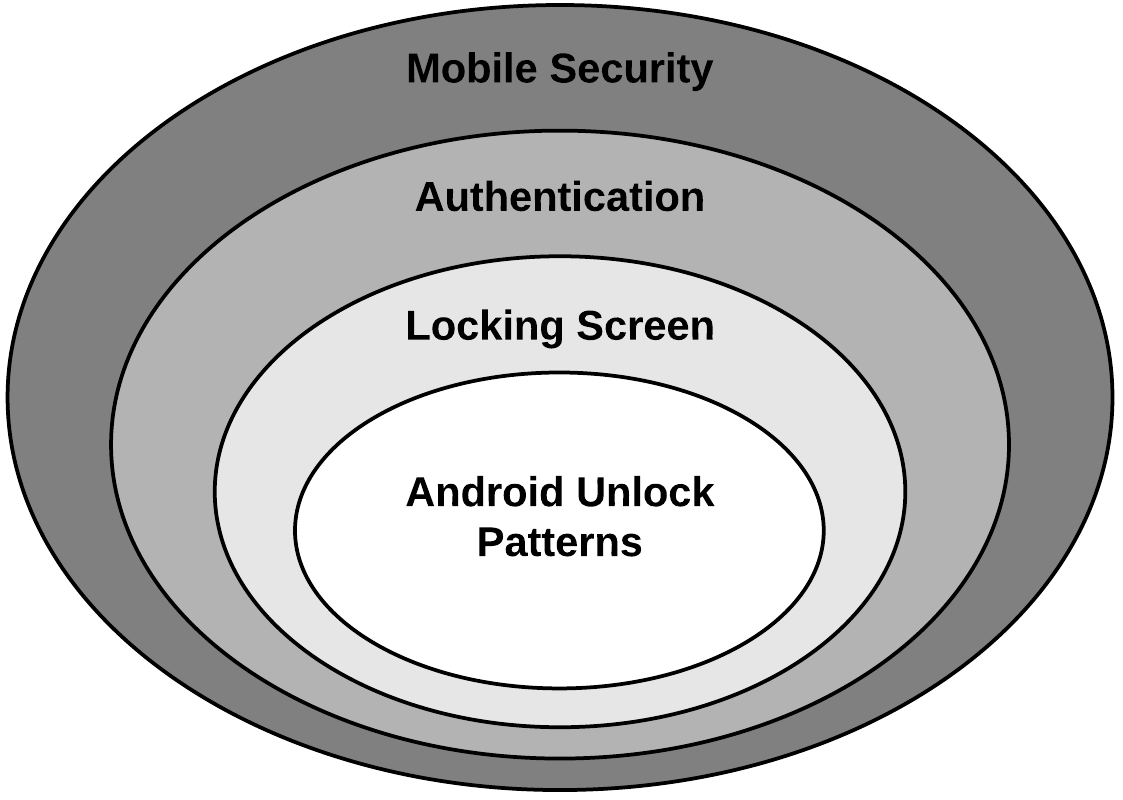
\includegraphics[scale=0.25]{pics/Fieldofstudy.png}
        \caption{Field of study}
      \end{figure}

    \subsection*{Keywords}  

      In the `field of study' I specified a specific scope in order to avoid to broad search space. 
      Inside each of the circles we can get more into details and create specific keywords that I will use in 
      the litterature search. 

      
        \begin{tabular}{ || l | l ||}
          \hline
          {\bf Mobile Security} & \\
          {\bf Locking Screen} &  \\
          {\bf Authentication} &  \\
          {\bf Android Unlock Patterns} & \\ 
          {\bf Psycology} & \\
          {\bf Graphical passwords} & \\
          \hline

          
        \end{tabular}




    \subsection*{Review Protocol}


